\documentclass{standalone}
\usepackage{tikz}
\usetikzlibrary{patterns, positioning}


\begin{document}
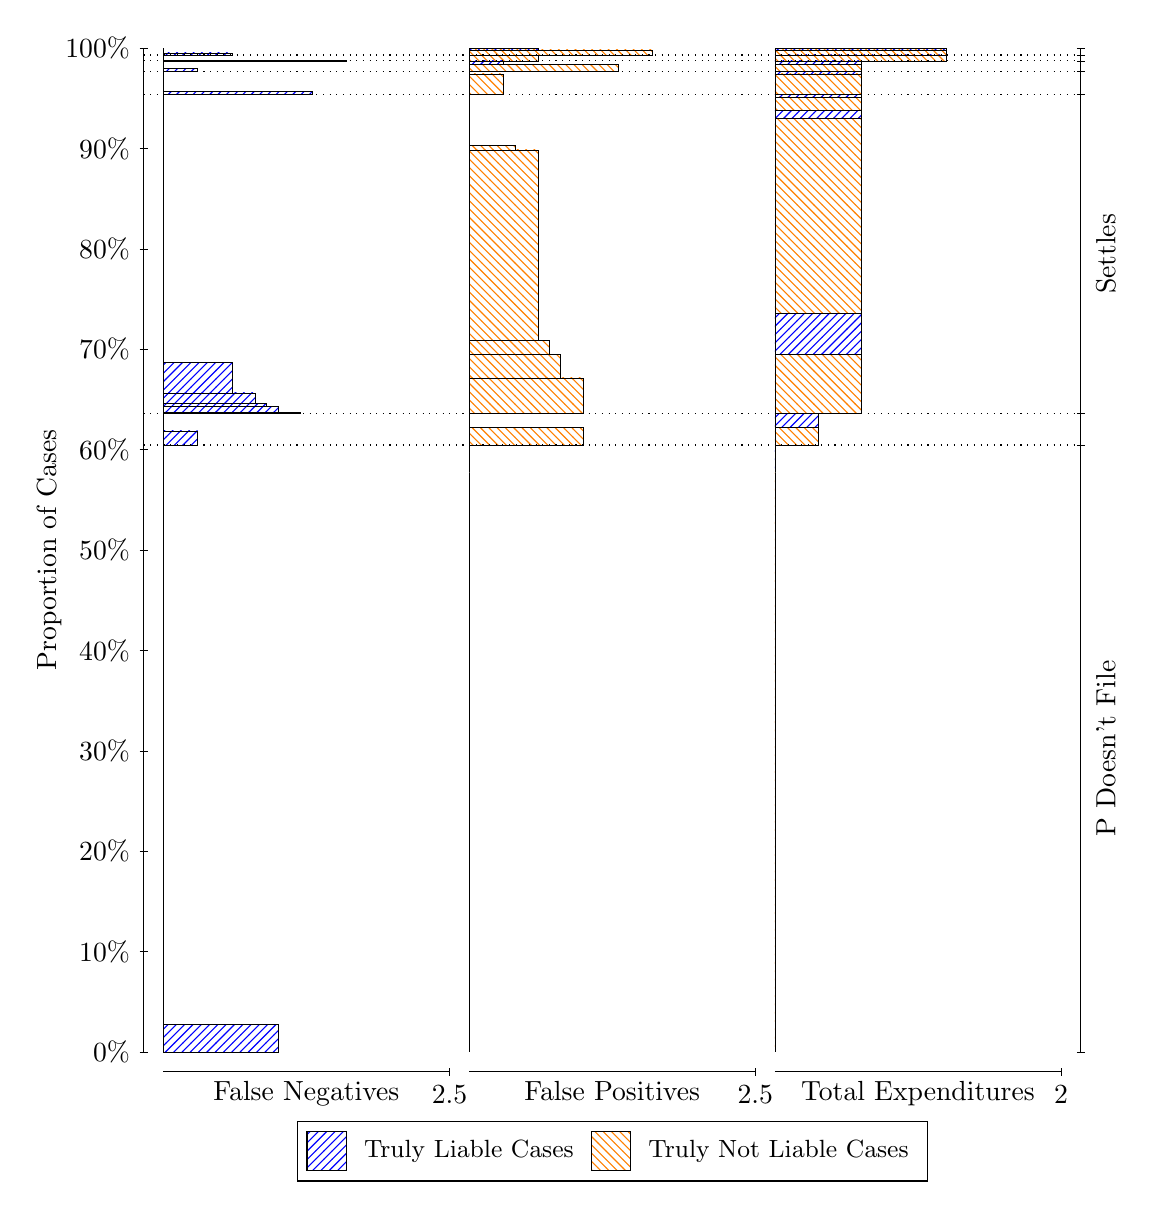
\begin{tikzpicture}
\draw[black, very thin] (1.5,1.75) -- (1.5,14.5);
\node[rotate=90, text=black, anchor=center] at (0.3, 8.125) {Proportion of Cases};
\draw[black, very thin] (1.45,1.75) -- (1.55,1.75);
\node[text=black, anchor=east] at (1.45, 1.75) {0\%};
\draw[black, very thin] (1.45,3.025) -- (1.55,3.025);
\node[text=black, anchor=east] at (1.45, 3.025) {10\%};
\draw[black, very thin] (1.45,4.3) -- (1.55,4.3);
\node[text=black, anchor=east] at (1.45, 4.3) {20\%};
\draw[black, very thin] (1.45,5.575) -- (1.55,5.575);
\node[text=black, anchor=east] at (1.45, 5.575) {30\%};
\draw[black, very thin] (1.45,6.85) -- (1.55,6.85);
\node[text=black, anchor=east] at (1.45, 6.85) {40\%};
\draw[black, very thin] (1.45,8.125) -- (1.55,8.125);
\node[text=black, anchor=east] at (1.45, 8.125) {50\%};
\draw[black, very thin] (1.45,9.4) -- (1.55,9.4);
\node[text=black, anchor=east] at (1.45, 9.4) {60\%};
\draw[black, very thin] (1.45,10.675) -- (1.55,10.675);
\node[text=black, anchor=east] at (1.45, 10.675) {70\%};
\draw[black, very thin] (1.45,11.95) -- (1.55,11.95);
\node[text=black, anchor=east] at (1.45, 11.95) {80\%};
\draw[black, very thin] (1.45,13.225) -- (1.55,13.225);
\node[text=black, anchor=east] at (1.45, 13.225) {90\%};
\draw[black, very thin] (1.45,14.5) -- (1.55,14.5);
\node[text=black, anchor=east] at (1.45, 14.5) {100\%};

\draw[black, very thin] (13.4,1.75) -- (13.4,14.5);
\draw[black, very thin] (13.35,1.75) -- (13.45,1.75);
\node[anchor=west] at (13.35, 1.75) {};
\draw[black, very thin] (13.35,9.4589) -- (13.45,9.4589);
\node[anchor=west] at (13.35, 9.4589) {};
\draw[black, very thin] (13.35,9.8613) -- (13.45,9.8613);
\node[anchor=west] at (13.35, 9.8613) {};
\draw[black, very thin] (13.35,13.91) -- (13.45,13.91);
\node[anchor=west] at (13.35, 13.91) {};
\draw[black, very thin] (13.35,14.207) -- (13.45,14.207);
\node[anchor=west] at (13.35, 14.207) {};
\draw[black, very thin] (13.35,14.336) -- (13.45,14.336);
\node[anchor=west] at (13.35, 14.336) {};
\draw[black, very thin] (13.35,14.412) -- (13.45,14.412);
\node[anchor=west] at (13.35, 14.412) {};
\draw[black, very thin] (13.35,14.5) -- (13.45,14.5);
\node[anchor=west] at (13.35, 14.5) {};

\draw[black, very thin, pattern color=blue, pattern=north east lines] (1.75,1.75) rectangle (3.2033,2.0967);
\draw[black, very thin, pattern color=orange, pattern=north west lines] (1.75,2.0967) rectangle (1.75,9.4589);
\draw[black, very thin, pattern color=blue, pattern=north east lines] (1.75,9.4589) rectangle (2.186,9.6365);
\draw[black, very thin, pattern color=orange, pattern=north west lines] (1.75,9.6365) rectangle (1.75,9.8613);
\draw[black, very thin, pattern color=blue, pattern=north east lines] (1.75,9.8613) rectangle (3.494,9.868);
\draw[black, very thin, pattern color=blue, pattern=north east lines] (1.75,9.868) rectangle (3.2033,9.9514);
\draw[black, very thin, pattern color=blue, pattern=north east lines] (1.75,9.9514) rectangle (3.058,9.9824);
\draw[black, very thin, pattern color=blue, pattern=north east lines] (1.75,9.9824) rectangle (2.9127,10.121);
\draw[black, very thin, pattern color=blue, pattern=north east lines] (1.75,10.121) rectangle (2.622,10.506);
\draw[black, very thin, pattern color=orange, pattern=north west lines] (1.75,10.506) rectangle (1.75,13.91);
\draw[black, very thin, pattern color=blue, pattern=north east lines] (1.75,13.91) rectangle (3.6393,13.945);
\draw[black, very thin, pattern color=orange, pattern=north west lines] (1.75,13.945) rectangle (1.75,14.207);
\draw[black, very thin, pattern color=blue, pattern=north east lines] (1.75,14.207) rectangle (2.186,14.245);
\draw[black, very thin, pattern color=orange, pattern=north west lines] (1.75,14.245) rectangle (1.75,14.336);
\draw[black, very thin, pattern color=blue, pattern=north east lines] (1.75,14.336) rectangle (4.0753,14.343);
\draw[black, very thin, pattern color=orange, pattern=north west lines] (1.75,14.343) rectangle (1.75,14.412);
\draw[black, very thin, pattern color=blue, pattern=north east lines] (1.75,14.412) rectangle (2.622,14.437);
\draw[black, very thin, pattern color=orange, pattern=north west lines] (1.75,14.437) rectangle (1.75,14.5);
\draw[black, very thin, pattern color=orange, pattern=north west lines] (5.6333,1.75) rectangle (5.6333,9.1121);
\draw[black, very thin, pattern color=blue, pattern=north east lines] (5.6333,9.1121) rectangle (5.6333,9.4589);
\draw[black, very thin, pattern color=orange, pattern=north west lines] (5.6333,9.4589) rectangle (7.0867,9.6837);
\draw[black, very thin, pattern color=blue, pattern=north east lines] (5.6333,9.6837) rectangle (5.6333,9.8613);
\draw[black, very thin, pattern color=orange, pattern=north west lines] (5.6333,9.8613) rectangle (7.0867,10.311);
\draw[black, very thin, pattern color=orange, pattern=north west lines] (5.6333,10.311) rectangle (6.796,10.61);
\draw[black, very thin, pattern color=orange, pattern=north west lines] (5.6333,10.61) rectangle (6.6507,10.785);
\draw[black, very thin, pattern color=orange, pattern=north west lines] (5.6333,10.785) rectangle (6.5053,13.206);
\draw[black, very thin, pattern color=orange, pattern=north west lines] (5.6333,13.206) rectangle (6.2147,13.266);
\draw[black, very thin, pattern color=blue, pattern=north east lines] (5.6333,13.266) rectangle (5.6333,13.91);
\draw[black, very thin, pattern color=orange, pattern=north west lines] (5.6333,13.91) rectangle (6.0693,14.171);
\draw[black, very thin, pattern color=blue, pattern=north east lines] (5.6333,14.171) rectangle (5.6333,14.207);
\draw[black, very thin, pattern color=orange, pattern=north west lines] (5.6333,14.207) rectangle (7.5227,14.297);
\draw[black, very thin, pattern color=blue, pattern=north east lines] (5.6333,14.297) rectangle (6.0693,14.336);
\draw[black, very thin, pattern color=orange, pattern=north west lines] (5.6333,14.336) rectangle (6.5053,14.405);
\draw[black, very thin, pattern color=blue, pattern=north east lines] (5.6333,14.405) rectangle (5.6333,14.412);
\draw[black, very thin, pattern color=orange, pattern=north west lines] (5.6333,14.412) rectangle (7.9587,14.475);
\draw[black, very thin, pattern color=blue, pattern=north east lines] (5.6333,14.475) rectangle (6.5053,14.5);
\draw[black, very thin, pattern color=orange, pattern=north west lines] (9.5167,1.75) rectangle (9.5167,9.1121);
\draw[black, very thin, pattern color=blue, pattern=north east lines] (9.5167,9.1121) rectangle (9.5167,9.4589);
\draw[black, very thin, pattern color=orange, pattern=north west lines] (9.5167,9.4589) rectangle (10.062,9.6837);
\draw[black, very thin, pattern color=blue, pattern=north east lines] (9.5167,9.6837) rectangle (10.062,9.8613);
\draw[black, very thin, pattern color=orange, pattern=north west lines] (9.5167,9.8613) rectangle (10.607,10.61);
\draw[black, very thin, pattern color=blue, pattern=north east lines] (9.5167,10.61) rectangle (10.607,11.133);
\draw[black, very thin, pattern color=orange, pattern=north west lines] (9.5167,11.133) rectangle (10.607,13.614);
\draw[black, very thin, pattern color=blue, pattern=north east lines] (9.5167,13.614) rectangle (10.607,13.704);
\draw[black, very thin, pattern color=orange, pattern=north west lines] (9.5167,13.704) rectangle (10.607,13.879);
\draw[black, very thin, pattern color=blue, pattern=north east lines] (9.5167,13.879) rectangle (10.607,13.91);
\draw[black, very thin, pattern color=orange, pattern=north west lines] (9.5167,13.91) rectangle (10.607,14.171);
\draw[black, very thin, pattern color=blue, pattern=north east lines] (9.5167,14.171) rectangle (10.607,14.207);
\draw[black, very thin, pattern color=orange, pattern=north west lines] (9.5167,14.207) rectangle (10.607,14.297);
\draw[black, very thin, pattern color=blue, pattern=north east lines] (9.5167,14.297) rectangle (10.607,14.336);
\draw[black, very thin, pattern color=orange, pattern=north west lines] (9.5167,14.336) rectangle (11.697,14.405);
\draw[black, very thin, pattern color=blue, pattern=north east lines] (9.5167,14.405) rectangle (11.697,14.412);
\draw[black, very thin, pattern color=orange, pattern=north west lines] (9.5167,14.412) rectangle (11.697,14.475);
\draw[black, very thin, pattern color=blue, pattern=north east lines] (9.5167,14.475) rectangle (11.697,14.5);
\draw[black, dotted] (1.5,9.4589) -- (13.4,9.4589);
\draw[black, dotted] (1.5,9.8613) -- (13.4,9.8613);
\draw[black, dotted] (1.5,13.91) -- (13.4,13.91);
\draw[black, dotted] (1.5,14.207) -- (13.4,14.207);
\draw[black, dotted] (1.5,14.336) -- (13.4,14.336);
\draw[black, dotted] (1.5,14.412) -- (13.4,14.412);
\draw[black, very thin] (1.75,1.5) -- (5.3833,1.5);
\node[text=black, anchor=north] at (3.5667, 1.5) {False Negatives};
\draw[black, very thin] (5.3833,1.45) -- (5.3833,1.55);
\node[text=black, anchor=north] at (5.3833, 1.45) {2.5};

\draw[black, very thin] (5.6333,1.5) -- (9.2667,1.5);
\node[text=black, anchor=north] at (7.45, 1.5) {False Positives};
\draw[black, very thin] (9.2667,1.45) -- (9.2667,1.55);
\node[text=black, anchor=north] at (9.2667, 1.45) {2.5};

\draw[black, very thin] (9.5167,1.5) -- (13.15,1.5);
\node[text=black, anchor=north] at (11.333, 1.5) {Total Expenditures};
\draw[black, very thin] (13.15,1.45) -- (13.15,1.55);
\node[text=black, anchor=north] at (13.15, 1.45) {2};

\node[text=black, centered, rotate=90] at (13.72, 5.6044) {P Doesn't File};

\node[text=black, centered, rotate=90] at (13.72, 11.886) {Settles};





\draw (7.449999999999999,1.5) node[draw=none] (baseCoordinate) {};
\begin{scope}[align=center]
        \matrix[scale=0.5, draw=black, below=0.5cm of baseCoordinate, nodes={draw}, column sep=0.1cm]{
            \node[rectangle, draw, minimum width=0.5cm, minimum height=0.5cm, pattern color=blue, pattern=north east lines] {}; &
            \node[draw=none, font=\small, text=black] (B) {Truly Liable Cases}; &
            \node[rectangle, draw, minimum width=0.5cm, minimum height=0.5cm, pattern color=orange, pattern=north west lines] {}; &
            \node[draw=none, font=\small, text=black] (B) {Truly Not Liable Cases}; \\
            };
\end{scope}

\end{tikzpicture}
\end{document}